% !Rnw weave = knitr
% !TeX program = XeLaTeX
\documentclass[final,a4paper,romanappendices]{IEEEtran}\usepackage[]{graphicx}\usepackage[]{color}
%% maxwidth is the original width if it is less than linewidth
%% otherwise use linewidth (to make sure the graphics do not exceed the margin)
\makeatletter
\def\maxwidth{ %
  \ifdim\Gin@nat@width>\linewidth
    \linewidth
  \else
    \Gin@nat@width
  \fi
}
\makeatother

\definecolor{fgcolor}{rgb}{0.345, 0.345, 0.345}
\newcommand{\hlnum}[1]{\textcolor[rgb]{0.686,0.059,0.569}{#1}}%
\newcommand{\hlstr}[1]{\textcolor[rgb]{0.192,0.494,0.8}{#1}}%
\newcommand{\hlcom}[1]{\textcolor[rgb]{0.678,0.584,0.686}{\textit{#1}}}%
\newcommand{\hlopt}[1]{\textcolor[rgb]{0,0,0}{#1}}%
\newcommand{\hlstd}[1]{\textcolor[rgb]{0.345,0.345,0.345}{#1}}%
\newcommand{\hlkwa}[1]{\textcolor[rgb]{0.161,0.373,0.58}{\textbf{#1}}}%
\newcommand{\hlkwb}[1]{\textcolor[rgb]{0.69,0.353,0.396}{#1}}%
\newcommand{\hlkwc}[1]{\textcolor[rgb]{0.333,0.667,0.333}{#1}}%
\newcommand{\hlkwd}[1]{\textcolor[rgb]{0.737,0.353,0.396}{\textbf{#1}}}%
\let\hlipl\hlkwb

\usepackage{framed}
\makeatletter
\newenvironment{kframe}{%
 \def\at@end@of@kframe{}%
 \ifinner\ifhmode%
  \def\at@end@of@kframe{\end{minipage}}%
  \begin{minipage}{\columnwidth}%
 \fi\fi%
 \def\FrameCommand##1{\hskip\@totalleftmargin \hskip-\fboxsep
 \colorbox{shadecolor}{##1}\hskip-\fboxsep
     % There is no \\@totalrightmargin, so:
     \hskip-\linewidth \hskip-\@totalleftmargin \hskip\columnwidth}%
 \MakeFramed {\advance\hsize-\width
   \@totalleftmargin\z@ \linewidth\hsize
   \@setminipage}}%
 {\par\unskip\endMakeFramed%
 \at@end@of@kframe}
\makeatother

\definecolor{shadecolor}{rgb}{.97, .97, .97}
\definecolor{messagecolor}{rgb}{0, 0, 0}
\definecolor{warningcolor}{rgb}{1, 0, 1}
\definecolor{errorcolor}{rgb}{1, 0, 0}
\newenvironment{knitrout}{}{} % an empty environment to be redefined in TeX

\usepackage{alltt}%draft, onecolumn,9pt,twoside
\usepackage[utf8]{inputenc}
\usepackage[T1]{fontenc}
\usepackage[spanish]{babel}
\spanishdatedel
\usepackage{amsmath,amsthm}
\usepackage[cmintegrals]{newtxmath}
\usepackage{bm}
\usepackage{graphicx}
\usepackage{algorithm}
\usepackage{algpseudocode}
\usepackage{lipsum}
\floatname{algorithm}{Algoritmo}

\theoremstyle{definition}
\newtheorem{definition}{Definición}[subsection]
\title{Un algoritmo aleatorizado para calcular la mediana}
\author{\IEEEauthorblockN{Erwin Talla Chumpitaz\IEEEauthorrefmark{1},
Carlos Aznarán Laos\IEEEauthorrefmark{2}, Miller Silva Menejes\IEEEauthorrefmark{3} y 
Jesús Jáuregui Alvarado\IEEEauthorrefmark{4}}
\IEEEauthorblockA{\\Facultad de Ciencias,
Universidad Nacional de Ingeniería\\
Av. Túpac Amaru 210, Rímac, Lima 25, Perú\\
Email: \IEEEauthorrefmark{1}erwinleo\textunderscore 98\MVAt hotmail.com,
\IEEEauthorrefmark{2}caznaranl\MVAt uni.pe,
\IEEEauthorrefmark{3}miller\textunderscore silva\textunderscore 96\MVAt hotmail.com,
\IEEEauthorrefmark{4}jjaureguia\MVAt uni.pe}}

\newcommand{\MVAt}{{\usefont{U}{mvs}{m}{n}\symbol{`@}}}
%\thanks{El profesor César Lara Ávila}
%\author{Michael \IEEEmembership{Member,~IEEE,\thanks{M}}}

%\renewcommand\IEEEkeywordsname{Palabras clave}
\IfFileExists{upquote.sty}{\usepackage{upquote}}{}
\begin{document}
\maketitle
%\begin{abstract}
%En este trabajo, 
% Una pequeña descripción total del trabajo.
%\end{abstract}
%\begin{IEEEkeywords}
%Cuantil, Percentil, Mediana, Quick Sort, Heap Sort.
%\end{IEEEkeywords}
% TODO: Después de introducción que esté en dos columnas.
\section{Introducción}
No hay persona en el mundo que no se haya valido en la Estadística y Probabilidad en algún momento de su vida, desde calcular el tiempo promedio al salir de su casa a esperar el bus para dirigirse al trabajo, pasando por juegos de azar, hasta realizar complejos cálculos para pronosticar resultados futuros para invertir en la bolsa. En el mundo de la estadística existen distintas medidas de tendencia central, entre las más comunes se encuentran; la media, la mediana y la moda, en este reporte nos enfocaremos en la Mediana, repasando desde su origen, importancia y sus aplicaciones en la vida, mediante un ejemplo con datos estadísticos recogidos desde (\textbf{Aún no se ha definido la muestra sobre la cual se va a realizar la experimentación}), entonces al finalizar de leer este reporte usted sabrá como y cuando utilizar la mediana como medida de tendencia central, así mismo le mostraremos como implementar un código en R que realice este procedimiento de la manera más eficientemente posible.
%\section{Definiciones}
% TODO: (JAUREGUI) Completar 
\begin{definition}[Percentil]
Es una medida de posición, donde Percentil i es aquel valor $P_{i}$ que deja a su izquierda el $i$ y el resto por encima de los valores de la muestra ordenada de menor a mayor, de esta forma el valor de la mediana es representada como el Percentil $50$,  $P_{50}$.
\end{definition}

\begin{definition}[Cálculo de percentiles (Caso Continuo)]

\begin{enumerate}
	\item Construir la tabla de porcentajes acumulados $P_{l}$.
	\item	Ubicar el $50$\% tal que: $$ P_{i-1} \leq l\leq P_{i} $$.
	\item $L_{i-1}$ y $L_{i}$ son los límites inferior y superior del intervalo correspondientes a $P_{i-1}$ y $P_{i}$ respectivamente.
\end{enumerate}
		
Entonces el percentil $p_{l}$ se calcula mediante la siguiente fórmula: $$ p_{l} = L_{i-1} + \frac{l - P_{i-1}}{P_{i} + P_{i-1}} (L_{i} - L_{i-1}).$$
\end{definition}
%\begin{definition}[Mediana de una distribución]
%Es un valor $x_m$ de $\mathbb{X}$ tal que el $50\%$ de los posibles valores de $X$ están por debajo de $x_m$ y el $50\%$ de los posibles valores de $\mathbb{X}$ están por arriba de $x_m$.
%\end{definition}

\section{Estado del arte}

\begin{itemize}
  \item El primer algoritmo aleatorizado fue un método desarrollado por Michael O. Rabin para el problema de par más cercano en la geometría computacional:

{\centering
``Dados n puntos en el espacio métrico , encuentre un par de puntos con la menor distancia entre ellos''\par
}
  \item Un algoritmo ingenuo para encontrar distancias entre todos los pares de puntos en un espacio de dimensión $d$ y seleccionar el mínimo requiere $O(n^2)$ tiempo y se puede resolver en $O(n\log n)$ tiempo en un espacio euclidiano. En el modelo computacional que
asume que la función de piso es computable en tiempo constante, el problema se puede resolver en el tiempo $O(n\log n\log n)$. Si permitimos que la aleatorización se use junto con la función de piso, el problema se puede resolver en el tiempo $O(n)$. 
  \item Michael O. Rabin demostró que la prueba de primalidad de Miller de 1976 se puede convertir en un algoritmo aleatorizado. En ese momento, no se conocía ningún algoritmo determinístico práctico para la primalidad.
  \item Actualmente existen varios algoritmos aleatorios para encontrar la mediana, cada algoritmo se diferencia en su procedimiento para ordenar los datos aleatorios. Los algoritmos más usados por su eficacia y eficiencia para ordenar datos son merge sort, heapsort y quicksort.
\end{itemize}

\section{Diseño del experimento}
En este proyecto, para obtener un algoritmo eficiente para obtener de manera aleatoria la mediana de un conjunto de datos desordenados, se debe tener algunos conceptos previos para poder entender y posteriormente desarrollar un código. Los conceptos a desarrollar son: Algoritmos de búsqueda, Algoritmos de ordenamiento, Algoritmos aleatorios.

\subsection{Algoritmos de búsqueda}
Un algoritmo de búsqueda se encarga de, a partir de una serie de criterios, encontrar un determinado elemento dentro de un conjunto de datos. Dentro de los más conocidos y más utilizados están:
\subsubsection{Búsqueda secuencial}
Para encontrar un elemento en un conjunto estructurado, se analiza elemento por elemento hasta encontrar con aquel elemento solicitado. Tiene un tiempo, en el peor caso, de $O(n)$.
\subsection{Búsqueda binaria}
En este caso, el conjunto de elementos debe estar ordenado de modo que se compara con el elemento medio si es menor(izquierda), mayor(derecha) e igual (devuelve el valor), y se repite el proceso reduciendo la cantidad de datos. Tiene un tiempo, en el peor caso, de $O(log2n)$.

\subsection{Algoritmo de ordenamiento}

Un algoritmo de ordenamiento se encarga de comparar todos los elementos y colocarlos en un orden, mediante algún método (intercambio, mezcla, partición, etc.). Los algoritmos más utilizados son: %(Cormen. 30-31, 148-150, 170-174)

\subsubsection{Ordenamiento de burbuja}

Este algoritmo funciona comparando cada elemento de la lista con el siguiente e intercambiando si es que el elemento comparado es menor. Tiene como complejidad $O(n^2)$.

\subsubsection{Ordenamiento por mezcla}

Este algoritmo funciona dividiendo en la mitad recursivamente en una cantidad de elementos, cuando son pequeñas cantidades se procede a ordenarlos y agruparlos, de manera progresiva hasta su totalidad. Tiene complejidad $O(n\log_{2} n)$.

\subsubsection{Ordenamiento rápido}

Este algoritmo funciona utilizando un pivote, el cual tiene la función de comparar y particionar el conjunto de datos entre menores y mayores que el pivote, este procedimiento se repite en las dos particiones y así sucesivamente. Tiene complejidad $O(n\log_{2} n)$. Es uno de los algoritmos más rápidos, por tal motivo se tiene pensado utilizar este algoritmo para lograr el objetivo de este proyecto.

\subsection{Algoritmos aleatorios}
Los algoritmos aleatorios son aquellos que utilizan en alguna parte de su estructura números aleatorios, con el fin de lograr las mismas posibilidades frente a cualquier caso. Es entonces, enfocado a nuestro proyecto, necesario utilizar la aleatoriedad para obtener una mejor probabilidad. Por lo expuesto, se procede a elaborar un seudocódigo para hallar la mediana de manera aleatoria con la idea de poder transcribirlo a cualquier lenguaje de programación, en nuestro caso en lenguaje R. Para hallar la mediana de un conjunto de datos, se deben de utilizar un algoritmo de ordenamiento y de búsqueda, ya que no se sabe si el conjunto de datos está ordenado. Para ello se analiza primero los algoritmos de búsqueda. Aplicado a nuestro objetivo sería ineficiente buscar secuencialmente la mediana, ya que no necesitamos recorrer toda la cadena para hallarlo, aun peor cuando no está ordenado. Igualmente pasaría con un algoritmo de búsqueda binaria, ya que de estar ordenado tan solo se necesitaría devolver. Entonces, es necesario implementar algún algoritmo de ordenamiento.
Como se presentó anteriormente, existen diferentes tipos de algoritmos de ordenamiento. Para escoger el más indicado se debe tomar en cuenta el tiempo de ejecución, es decir cuánto tiempo demora en ordenar todo el conjunto de datos. Para ello se utiliza la gran $O$ como determinante para el análisis de los tiempos. Se tiene algoritmos de ordenamiento en $O(n^2)$, $O(n\log_{2}n)$ y hasta $O(n)$. 
Sin embargo, no es necesario ordenarlo todo para hallarlo. Para ello se podría ordenar hasta $n/2$ de forma secuencial sin problema alguno y el resto dejarlo tal como estaba. Podría ser una solución buena, pero se puede mejorar aún más. Si analizamos la estructura del Quicksort, nos puede ayudar en la búsqueda de la mediana, el cual cuenta con dos funciones:
*La función ``PARTICION'' tiene como entrada $A$, $p$ y $r$. $A$ es una cadena de elementos de tamaño $n$, $p$ es la posición inicial relativa y $r$ es una posición final relativa. La función se encarga de seleccionar un pivote, el cual es el último elemento en la cadena, en donde se una separación de los números en comparación con el pivote, donde los menores irán a la izquierda y los mayores a la derecha. Por último, el pivote intercambia de posición con el primer mayor encontrado, y devuelve esa posición.

%\begin{algorithm}[ht]
%	\caption{Épsilon de la máquina}
%	\begin{algorithmic}[1]
%		\For{k}{1}{100}
%		\State $s \gets  0.5*s$
%		\State $t \gets s+1.0$
%		\If{ $t \leq 1.0$ }
%		\State $s \gets 2.0*s$
%		\State Escribir $k-1$, $s$
%		\State Salir
%		\EndIf
%		\EndFor
%	\end{algorithmic}
%\end{algorithm}

%\section{Agradecimientos}

\begin{knitrout}
\definecolor{shadecolor}{rgb}{0.969, 0.969, 0.969}\color{fgcolor}\begin{kframe}
\begin{alltt}
\hlkwd{set.seed}\hlstd{(}\hlnum{1121}\hlstd{)}
\hlstd{(x}\hlkwb{=}\hlkwd{rnorm}\hlstd{(}\hlnum{20}\hlstd{))}
\end{alltt}
\begin{verbatim}
##  [1]  0.1449583  0.4383221  0.1531912  1.0849426  1.9995449 -0.8118832
##  [7]  0.1602680  0.5858923  0.3600880 -0.0253084  0.1508809  0.1100824
## [13]  1.3596812 -0.3269946 -0.7163819  1.8097690  0.5084011 -0.5274603
## [19]  0.1327188 -0.1559430
\end{verbatim}
\begin{alltt}
\hlkwd{mean}\hlstd{(x);}\hlkwd{var}\hlstd{(x)}
\end{alltt}
\begin{verbatim}
## [1] 0.3217385
## [1] 0.5714534
\end{verbatim}
\end{kframe}
\end{knitrout}

The first element of \texttt{x} is 0.1449583. Boring boxplots
and histograms recorded by the PDF device:

\begin{knitrout}
\definecolor{shadecolor}{rgb}{0.969, 0.969, 0.969}\color{fgcolor}\begin{kframe}
\begin{alltt}
\hlcom{## two plots side by side (option fig.show='hold')}
\hlkwd{par}\hlstd{(}\hlkwc{mar}\hlstd{=}\hlkwd{c}\hlstd{(}\hlnum{4}\hlstd{,}\hlnum{4}\hlstd{,}\hlnum{.1}\hlstd{,}\hlnum{.1}\hlstd{),}\hlkwc{cex.lab}\hlstd{=}\hlnum{.95}\hlstd{,}\hlkwc{cex.axis}\hlstd{=}\hlnum{.9}\hlstd{,}\hlkwc{mgp}\hlstd{=}\hlkwd{c}\hlstd{(}\hlnum{2}\hlstd{,}\hlnum{.7}\hlstd{,}\hlnum{0}\hlstd{),}\hlkwc{tcl}\hlstd{=}\hlopt{-}\hlnum{.3}\hlstd{,}\hlkwc{las}\hlstd{=}\hlnum{1}\hlstd{)}
\hlkwd{boxplot}\hlstd{(x)}
\end{alltt}
\end{kframe}
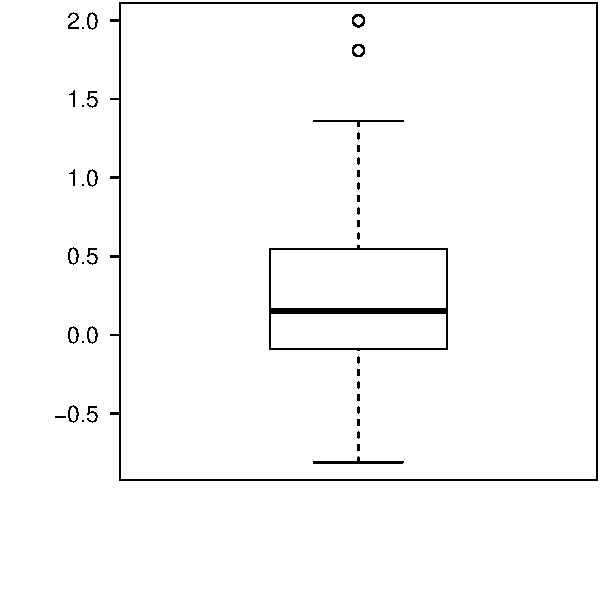
\includegraphics[width=.4\linewidth]{figure/boring-plots-1} 
\begin{kframe}\begin{alltt}
\hlkwd{hist}\hlstd{(x,}\hlkwc{main}\hlstd{=}\hlstr{''}\hlstd{)}
\end{alltt}
\end{kframe}
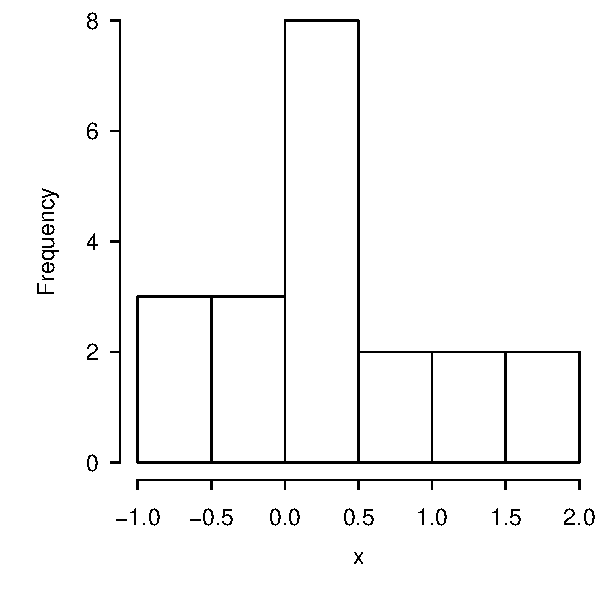
\includegraphics[width=.4\linewidth]{figure/boring-plots-2} 

\end{knitrout}
\end{document}
Buscar los método de contraste de mediana y moda.
